\chapter{SystemNaim: Design Decisions}

Since SystemNaim is a tool with many parts needing to be implemented, each aspect of the tool had different motivations and goals. For some parts we focused on getting a working product and for others we focused on optimality, so that the end result was a tool which allowed to perform a full investigation of our aims. The following sections will go through the goals for each major segment of SystemNaim and discuss what we hoped that segment would contribute to the final tool.

\section{HLS}
\label{sec:hls_design}

The HLS aspect of SystemNaim is its backbone, it's how the users implement their own multi-FPGA systems, and thus it's focus had to be on usability. ANSI C90 was our input language of choice, due to both its simplicity and widespread knowledge of its syntax. Anyone who understands the basic concepts of programming: variables, loops and functions, would be able to pick C90 in less than a few minutes. Its simple grammar also means the HLS tool also becomes more straightforward. This is important because while the HLS tool is integral to SystemNaim it is also an aspect which could take up the entire development time if not limited in scope. 

Creating a competitive HLS tool would take years, but we didn't need a tool which rivalled Vivado HLS or LegUp, instead we just needed something that would allow us to prove we could automate the creation of a multi-FPGA system. Therefore, the HLS aspect of SystemNaim did not need to implement any hardware optimizations or even the full C90 feature set, it just needed to create functional hardware.

While optimizations were not a major concern, usability was. It needed to be easy for a user to designate which parts of the system they wanted to run on and off-chip, and it was therefore decided to use functions as a way of giving users control of hardware placement. The concept of a function is taught to every software engineer, it's a method of dividing the code base into smaller understandable chunks as well as avoiding code re-use, and in many ways share's similarities to hardware modules. Therefore, making the user decide where parts of the program would be run through the use of functions, is both intuitive for the user and simpler to implement for the tool. 

In order to do this, it was decided that C90 grammar would be expanded so that constructs, which allows the user to specify which functions to run in parallel and off-chip, could be added. Two new additions were decided upon, the “split” and “split\_fgpa” constructs. The former lets the user state which functions should be run in parallel instead of sequentially, while the latter allows the user to dictate which functions should be run on off-chip. To illustrate their usage, the grammar for the “split” and “split\_fgpa” constructs is as follows:

\begin{grammar}
    <split-function-call> ::= 'split' '\{' <split-list> '\}'
    \alt 'split\_fpga' '\{' <split-list> '\}'

    <split-list> ::= <split-item>
    \alt <split-list> <split-item>

    <split-item> ::= IDENTIFIER <assignment-operator> IDENTIFIER '(' argument-expression-list ')' ';'
\end{grammar}

For conciseness, the grammar rules have been merged into one, however in actual implementation there are two sets of rules for each construct in order for the right node classes to be instantiated. As can be seen the rules for $<split-item>$ are designed to be an assignment expression with only a function call on the right-hand side.

Additionally, \autoref{fig:new_constructs} shows how each of the constructs would be used in code.

\begin{figure}[H]
\centering

\begin{subfigure}{0.45\textwidth}
    \begin{minted}{Verilog}
split{
    holda = func_a(h, n/2);
    holdb = func_b(h, (n/2-1));
}
    \end{minted}
\end{subfigure}
\begin{subfigure}{0.45\textwidth}
    \begin{minted}{Verilog}
split_fpga{
    holda = func_a(h, n/2);
    holdb = func_b(h, (n/2-1));
}
    \end{minted}
\end{subfigure}
\begin{subfigure}{0.38\textwidth}
    \centering
    \begin{minted}{c}
holda = func_a(h, n/2);
holdb = func_b(h, (n/2-1));
    \end{minted}
\end{subfigure}
\caption{Usage of the new constructs added in SystemNaim, compared to conventional function calls.}
\label{fig:new_constructs}
\end{figure}

In summary, the HLS had the following requirements:

\begin{itemize}
    \item Have a low learning curve for users who have experience in software development.
    \item Allow users to designate the computation that occurs on each FPGA through functions and additional grammar.
    \item Not implement the full C90 feature set to reduce development time of the HLS tool.
\end{itemize}

\section{Interconnect}
\label{sec:interconnect_design}

The interconnect acts as the interface between the communication channel and the hardware generated by the HLS. It takes data from the HLS and passes it to the child FPGAs so that they can begin their processing. Without the interconnect, the HLS would have to directly control the channel which would require complex HDL to be generated every time the tool was run. By instead designing custom hardware, with a simple interface, the HLS can communicate with the interconnect thus resulting in simpler hardware being generated.

In essence, the interconnect forms a layer of abstraction between the HLS and the communication channel, so that the HLS tool does not require knowledge on how to control the channel in order to use it, thus lending towards the interconnect being modular in nature, which was one of the main goals we had when designing the hardware. We wanted the interconnect to act a form of abstraction in both directions; the HLS should have no knowledge of the channel, as mentioned, and the channel should have no knowledge of the HLS tool. With the intended result being that the interconnect could be used with any combination of HLS tool and communication channel.

This was done because the interconnect is the most important part of this project. Its design decides: how each FPGA communicates with each other, what the extra latency of the system is, what limitations are there for the off-chip processing? Therefore, it seemed like a waste to design custom hardware which could only be used in a single system. Instead, if we created a specification which could interface with multiple communication channels and had the potential to work with multiple HLS tools, we would have made something that could be used in other projects and could act as inspiration for future multi-FPGA system.

To be concise the interconnect requirements were as follows:

\begin{itemize}
    \item Interface with both the HLS generated HDL and the communication channel to act as a layer of abstraction between the two.
    \item Be modular in nature, so that different communication protocols can be used if the system requires it.
    \item Not to introduce so much latency to the system as to overshadow the benefit of off-loading processing to another FPGA.
\end{itemize}

\section{Communication Channel}

The communication channel was the area of SystemNaim we had the least control over, it would have been to large an undertaking to create our own protocol, and thus we had to choose from a set of pre-existing ones. What we were looking for was that had a high channel bandwidth but low protocol complexity. By protocol complexity, we mean how many additional bits are sent over the channel besides the actual payload that we are trying to transmit.

The higher the protocol complexity the more bits are being sent on every transaction and thus make each one take longer. Ethernet is a good example of a protocol which has a high amount of overhead, but also very fast bandwidth. Each transaction may have 50 bytes of overhead data, which ends up increasing the latency of the resulting system, however, Ethernet can also run at very high bandwidths, so this additional overhead can be mitigated when compared to other protocols.

At it's core the communication channel just needs to allow each FPGA to send and receive data, therefore it didn't matter too much about which one we chose. In addition, with the interconnect being designed in a such a way where the channel protocol could be changed later on without requiring a total overhaul of SystemNaim, we were able to pick the protocol that was the easiest to implement. The channel protocol could then, in the future, be chosen according to a user's bandwidth needs and port availability.

\section{The System as a Whole}
\label{sec:full_system}

SystemNaim is designed to be able to generate a 2-FPGA system, with one parent and one child FPGA. The parent FPGA contains the main parts of the program, and during operation it can make remote calls, similar to an RPC system, to the child FPGA. The child FPGA contains off-chip functions, which are hardware modules that perform the processing of one function, when the child FPGA receives a remote call it will begin execution and once complete it will pass the result back to the parent FPGA. \autoref{fig:full_sys} shows a high level view of what a multi-FPGA system generated by SystemNaim would look like.

\begin{figure}[!htb]
    \centering
    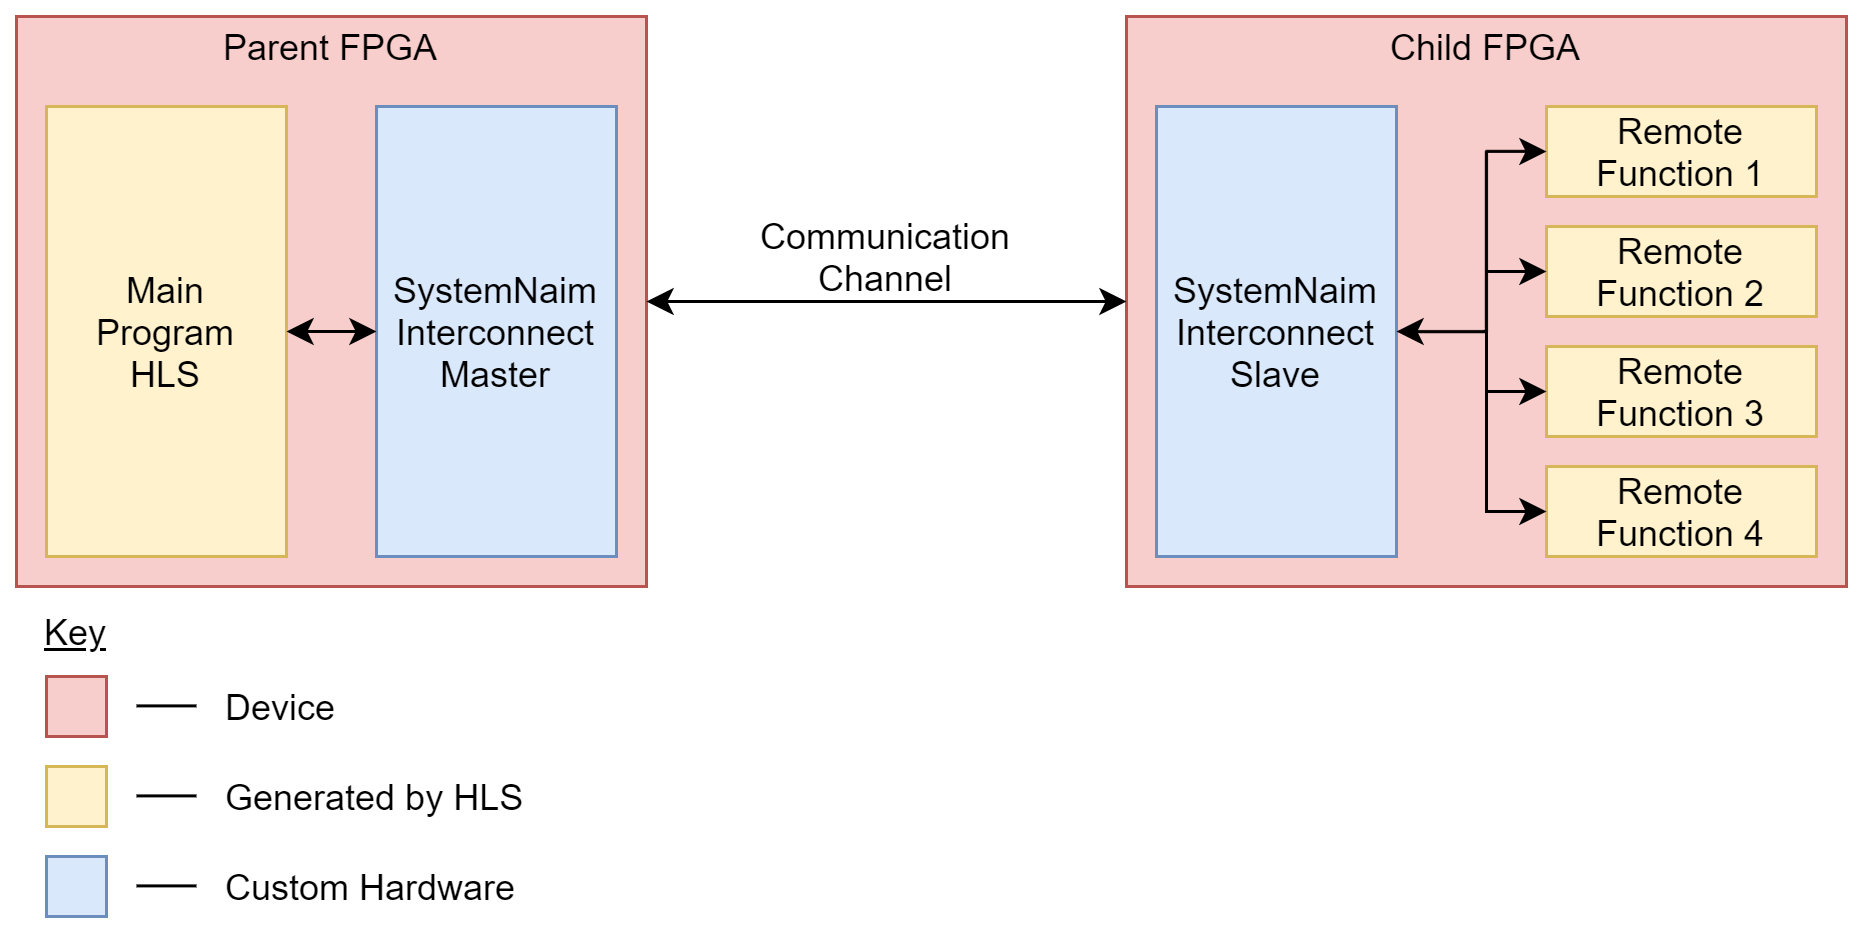
\includegraphics[width=0.9\textwidth]{03_design/images/full_system.png}
    \caption{Basic multi-FPGA system generated by SystemNaim}
    \label{fig:full_sys}
\end{figure}

To make it easier to understand the usage of the SystemNaim a design flow graph has been created, \autoref{fig:design_flow}. As can be seen, the user needs to provide input files, and then, using Quartus and the NIOS II development tools, load their system onto an FPGA.

\begin{sidewaysfigure}[!htb]
    \centering
    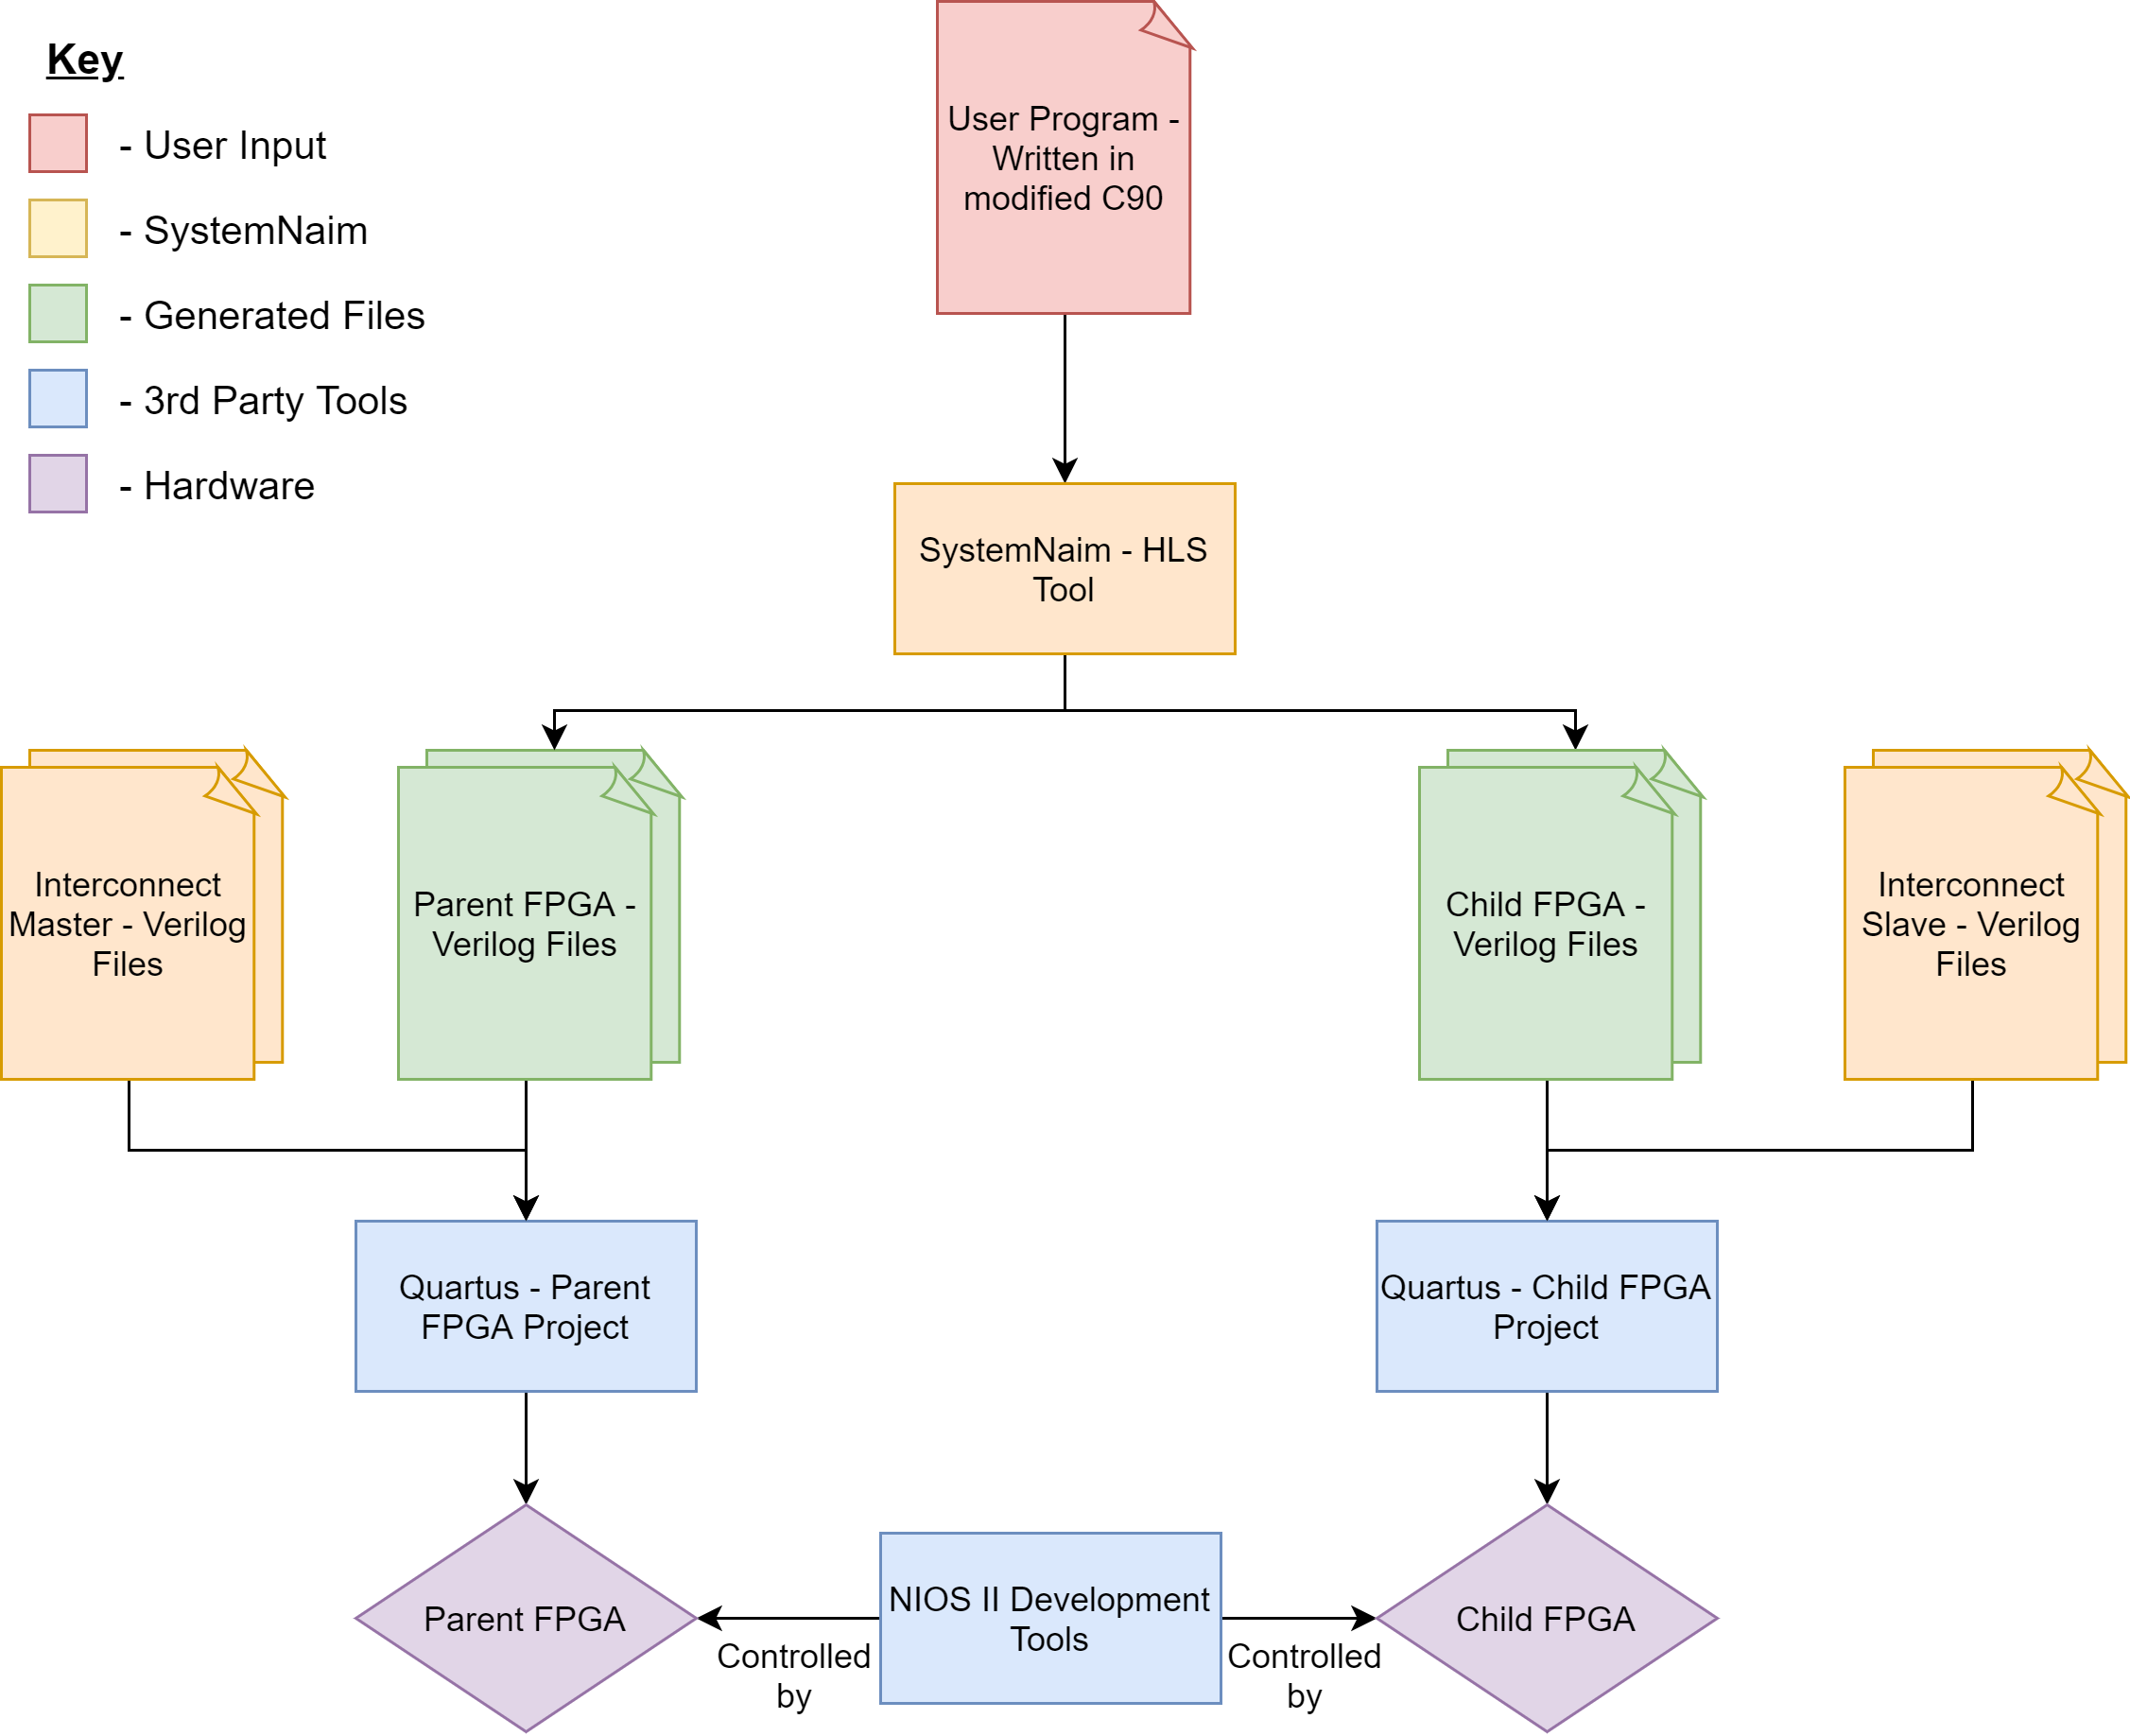
\includegraphics[width=0.9\textwidth]{03_design/images/design_flow.png}
    \caption{Design Flow of a system when using SystemNaim}
    \label{fig:design_flow}
\end{sidewaysfigure}